\section{Analisi Dei Componenti}
In questo capitolo viene descritta l'architettura interna del sistema JGuesser. La presentazione dell'architettura interna avviene individuando le diverse componenti, che costituiscono il sistema, e specificando i flussi di dati in ingresso e in uscita individuati all'interno del diagramma di contesto. L'identificazione quindi delle componenti, l'interazione che essi hanno tra di loro e quindi i dati che devono scambiarsi e la specificazione dei flussi in entrata ed in uscita al sistema, permettono quindi di definire il diagramma delle componenti. 

\subsection{Definizione dei componenti}
In questa sezione vengono definiti i componenti che formeranno il sistema JGuesser. In particolare ne viene motivata la loro esistenza, attraverso dei riferimenti ai requisiti funzionali e vengono spiegate le interfacce fornite o richieste. 

\subsubsection{Pagina registrazione}
\textbf{Descrizione: }questo componente si occupa di permettere all'utente di inserire le diverse informazioni per registrarsi e di inviare al componente validatore reCAPTCHA il proprio reCAPTCHA token. Oltre a ciò si occupa di verificare che il formato dei dati sia quello corretto. Questo componente è stato creato per rispondere al requisito funzionale \ref{req_registrazione}. \\
\\
\textbf{Interfaccia richiesta – Info registrazione: }per informazioni di registrazione si intendono:
\begin{itemize}
    \item Username
    \item E-mail
    \item Password
    \item Conferma password
    \item Nazione
\end{itemize}
\noindent
\textbf{Interfaccia richiesta – reCAPTCHA token: }cliccando sul reCAPTCHA presente nella pagina di registrazione, l'utente genera una chiave, che dovrà essere validato dal sistema esterno reCAPTCHA. \\
\\
\textbf{Interfaccia fornita – reCAPTCHA token: }la chiave del reCAPTCHA deve essere inviata alla componente validatore reCAPTCHA, che si occuperà di effettuare la validazione. \\
\\
\textbf{Interfaccia fornita – Info registrazione: }vengono inoltrare le informazioni di registrazione alla componente gestore credenziali. \\
\\
\textbf{Interfaccia richiesta – Check registrazione: }flag di registrazione, che vale 'false' nel caso in cui si sia verificato qualche errore durante la registrazione. Serve a mostrare eventuali messaggi d'errore.

\subsubsection{Gestore registrazione}
\textbf{Descrizione: }dato il RF\ref{req_registrazione}, l'applicazione deve fornire all'utente la possibilità di registrarsi. Per questo motivo è stato definito un componente che si occupa di verificare e attuare la registrazione. Questa componente si occupa quindi di controllare che l'utente abbia inserito tutti i dati necessari e che questi rispettino alcuni vincoli. Oltre a ciò attuerà la registrazione interrogando il database e restituirà un check di conferma/errore alla componente di pagina di registrazione.  \\
\\
\textbf{Interfaccia fornita – Check registrazione: }flag di registrazione che sarà generato dalla componente gestore registrazione. Questo flag varrà 'true' se il Check reCAPTCHA e il Check e-mail sono anche essi positivi e se valgono una serie di controlli effettuati all'interno di questa componente, es: non esiste alcun utente registrato con la stessa e-mail inserita dall'utente. \\
\\
\textbf{Interfaccia fornita – e-mail: }dato che verrà fornito all'interfaccia Nodemailer, che si occuperà di comunicare con il sistema esterno Nodemailer per verificare che l'e-mail sia una e-mail esistente e per sapere a quale indirizzo deve inviare l'e-mail di avvenuta registrazione, nel caso l'operazione di registrazione vada a buon fine. \\
\\
\textbf{Interfaccia fornita – Richiesta inserimento info registrazione:} viene inviata la richiesta d'inserimento dei dati di registrazione al sistema esterno MongoDB. \\
\\
\textbf{Interfaccia richiesta – Info registrazione:} la componente gestione registrazione riceve tutte le informazioni di registrazione che sono state raccolte dalla pagina di registrazione. \\
\\
\textbf{Interfaccia richiesta – Check e-mail:} valore che il gestore della registrazione riceverà dalla componente interfaccia Nodemailer e che serve a capire se l'e-mail inserita dall'utente è un e-mail valida oppure no. \\
\\
\textbf{Interfaccia richiesta – Check inserimento dati: }verifica da parte del sistema esterno MongoDB, che l'utente è stato registrato correttamente. Potrebbe verificarsi che per l'e-mail che l'utente ha specificato sia già esistente un profilo registrato. \\
\\
\textbf{Interfaccia richiesta – Credenziali google per registrazione: }insiemi di dati che si ricevono dalla componente autenticazione con google che servono a registrare l'utente all'interno del database nel caso in cui sia la prima volta che sta effettuando l'accesso con google.\\
\\
\textbf{Interfaccia richiesta – Check validazione reCAPTCHA: }valore che verrà ricevuto dalla componente validatore reCAPTCHA e che servirà alla componente gestore registrazione per capire se l'utente ha cliccato sul reCAPTCHA oppure no e quindi si è validato correttamente come non bot.\\
\\

\subsubsection{Validatore reCAPTCHA}
\textbf{Descrizione:} questa componente si occupa di verificare il reCAPTCHA token che l'utente invia al server. Il server deve infatti potersi interfacciare con il sistema esterno reCAPTCHA per capire se l'utente ha confermato correttamente la sua identità oppure no. Questo componente permette di realizzare i RF\ref{req_recupero_nome_utente_e_password} e RF\ref{req_registrazione}. \\
\\
\textbf{Interfaccia richiesta – reCAPTCHA token:} la componente validatore reCAPTCHA riceve dall'utente il reCAPTCHA token che dovrà essere validato. \\
\\
\textbf{Interfaccia richiesta – Check reCAPTCHA:} il sistema esterno reCAPTCHA restituisce alla componente validatore reCAPTCHA un dato, che permette di capire se la validazione è avvenuta con successo oppure no. \\
\\
\textbf{Interfaccia fornita – reCAPTCHA secret key:} il server invia al sistema esterno reCAPTCHA il proprio reCAPTCHA secret key, che servirà per poter verificare il reCAPTCHA token. \\
\\
\textbf{Interfaccia fornita – Check reCAPTCHA:} il dato che permette di capire la validità del reCAPTCHA viene inoltrato alle componenti: gestore registrazione e gestore credenziali a secondo di chi lo sta utilizzando in quel momento. \\
\\

\subsubsection{Interfaccia Nodemailer}
\textbf{Descrizione:} questa componente è quella che si interfaccia con il sistema esterno Nodemailer. È stata realizzata un unica componente, perché il sistema di invio e-mail è un sistema che cambia frequentemente ed è utile incapsulare tutte le interazioni in un unica componente. Questa componente risponde ai requisiti funzionali RF\ref{req_registrazione}, RF\ref{req_profilo_premium} e RF\ref{req_recupero_nome_utente_e_password}. \\
\\
\textbf{Interfaccia richiesta – Check e-mail:} l'interfaccia Nodemailer riceverà dal sistema esterno un dato che li permetterà di capire se l'e-mail inserita dall'utente è un e-mail esistente e quindi valida oppure no. \\
\\
\textbf{Interfaccia richiesta – e-mail:} l'interfaccia Nodemailer può ricevere un e-mail grazie al quale si dovranno eseguire delle operazioni da parte delle componenti: gestore registrazione, gestore credenziali e gestore upgrade profilo. \\
\\
\textbf{Interfaccia fornita – Richiesta verifica e-mail:} viene fornita al sistema esterno Nodemailer l'email di cui verificare l'esistenza. \\
\\
\textbf{Interfaccia fornita – Check e-mail:} il dato se l'e-mail è valida oppure no viene inoltrato alla componente di gestore registrazione. \\
\\
\textbf{Interfaccia fornita – Invio e-mail conferma registrazione:} viene inviata a Nodemailer una richiesta di inviare un e-mail all'utente che si è appena registrato, in cui viene avvisato di ciò. \\
\\
\textbf{Interfaccia fornita – Invio e-mail reset credenziali:} viene inviata a Nodemailer una richiesta di inviare un e-mail all'utente, che ha richiesto di resettare la propria password. L'utente riceverà quindi una e-mail con all'interno il proprio username e una nuova password generata casualmente. \\
\\
\textbf{Interfaccia fornita – Invio e-mail ringraziamento upgrade profilo:} viene inviata a Nodemailer una richiesta di inviare un e-mail di ringraziamento all'utente, che ha appena effettuato l'upgrade del proprio profilo alla versione premium. \\
\\

\subsubsection{Pagina login}
\textbf{Descrizione:} questa componente rappresenta l'interfaccia di login del sistema JGuesser. Ha quindi il compito di raccogliere le informazioni di login, verificare errori di formati delle credenziali e mostrare all'utente eventuali messaggi di errore che si possono verificare durante questa fase. Questa componente contribuisce a soddisfare i requisiti funzionali RF\ref{req_login_con_google} e RF\ref{req_login_con_credenziali}. \\
\\
\textbf{Interfaccia richiesta – One time code di google:} nel caso in cui l'utente abbia scelto di effettuare il login con google, otterrà un one time code che invierà alla componente di autenticazione con google. \\
\\
\textbf{Interfaccia richiesta – Credenziali:} l'utente inserisce nella pagina le proprie credenziali, per effettuare l'accesso. \\
\\
\textbf{Interfaccia richiesta – Check login google:} la pagina di login riceve dalla componente autenticazione con google un dato, che permetterà di capire se l'accesso con google è avvenuto con successo oppure no. \\
\\
\textbf{Interfaccia richiesta – Check login:} la pagina di login riceve dalla componente autenticazione un dato, che permetterà di capire se il login tramite credenziali è avvenuto con successo oppure no. \\
\\
\textbf{Interfaccia fornita – One time code di google:} viene inviato il one time code ottenuto dall'utente alla componente autenticazione con google.\\
\\
\textbf{Interfaccia fornita – Credenziali:} vengono inviate le credenziali di login alla componente autenticazione. \\
\\

\subsubsection{Autenticazione}
\textbf{Descrizione:} questa componente si occuperà di verificare l'autenticazione tramite le credenziali inserite dall'utente. Questa componente risponde al requisito funzionale RF\ref{req_login_con_credenziali}. \\
\\
\textbf{Interfaccia richiesta – Credenziali:} riceve le credenziali dalla componente pagina login. \\
\\
\textbf{Interfaccia richiesta – Password utente:} viene richiesto all'utente di inserire la propria password, che verrà poi verificata con quella associata all'username inserito all'interno del database. \\
\\
\textbf{Interfaccia fornita – Check login:} dato che viene restituito alla pagina di login, che indica se l'autenticazione ha avuto successo oppure no. \\
\\
\textbf{Interfaccia fornita – Richiesta password utente:} la componente interagirà con il sistema esterno MongoDB per inviare una richiesta di password dell'username inserito dall'utente. \\
\\

\subsubsection{Autenticazione con Google}
\textbf{Descrizione:} questa componente serve a gestire le interazioni con il sistema esterno google identity service e ad effettuare il login con google. Questa componente risponde al requisito funzionale RF\ref{req_login_con_google}. \\
\\
\textbf{Interfaccia richiesta – Info google:} questa componente interagirà con il sistema esterno google identity service, che fornirà:
\begin{itemize}
    \item access token;
    \item id token;
    \item e-mail.
\end{itemize}
\noindent
\textbf{Interfaccia richiesta – One time code di google:} riceve il one time code di google dalla pagina di login e quindi dall'utente. \\
\\
\textbf{Interfaccia fornita – Credenziali google per registrazione:} nel caso in cui sia la prima volta che un utente effettua l'accesso con google, le informazione che vengono restituite servissero per registrare un account per l'utente. \\
\\
\textbf{Interfaccia fornita – One time code di google:} si interagisce con il google identity service fornendoli il one time code.\\
\\
\textbf{Interfaccia fornita – Check login google:} si restituisce alla pagina di login un dato, che permetterà di capire se l'accesso con account google è avvenuto con successo oppure no. \\
\\

%GOLDO DEVE FARE FINO A QUI
\subsubsection{Pagina dati personali}
\textbf{Descrizione:} questo componente si occupa di permettere la modifica e la visualizzazione dei dati personali da parte dell’utente. I dati personali visualizzabili saranno: nazionalità, username e indirizzo mail. I dati modificabili saranno: indirizzo mail e password, per la modifica della prima sarà necessario inserire una mail, esistente e non associata ad un ulteriore account, sostitutiva. Per la modifica della password sarà necessario inserire la password attuale e la nuova password (che dovrà rispettare le stesse condizioni della fase di registrazione) per 2 volte. All’interno di questa componente verrà effettuato un controllo di uguaglianza tra le 2 nuove password inserite e, in caso di esito positivo del confronto, verrà inviata la prima di queste due più la vecchia password alla componente Gestore credenziali. Questo componente è stato creato per rispondere ai requisiti funzionali RF\ref{req_visualizzazione_dati_personali}, RF\ref{req_modifica_e-mail} e RF\ref{req_modifica_password}. \\
\\
\textbf{Interfaccia richiesta – Nuove credenziali:} vengono richieste all’utente le nuove credenziali, ovvero il nuovo indirizzo e-mail in caso si voglia modificare quest’ultima, altrimenti la nuova password per 2 volte, sarà poi la componente stessa che verificherà la corrispondenza tra le due. \\
\\
\textbf{Interfaccia richiesta – Vecchia password:} viene richiesto all’utente di inserire la vecchia password, utilizzata per permettere la modifica della stessa, tale password verrà poi inoltrata al Gestore credenziali, che si occuperà di accertarne la validità. \\
\\
\textbf{Interfaccia richiesta – Check modifica credenziali:} viene richiesta una conferma da parte del Gestore credenziali dell’avvenuta modifica delle credenziali. \\
\\
\textbf{Interfaccia richiesta – Dati utente:} vengono richiesti dal Gestore credenziali i dati utente da visualizzare nelle informazioni personali, tali dati saranno poi mostrati all’utente. \\
\\
\textbf{Interfaccia fornita – Informazioni dati personali:} vengono mostrati all’utente i propri dati personali. \\
\\
\textbf{Interfaccia fornita – Nuove credenziali:} viene fornita al Gestore credenziali la nuova credenziale inserita dall’utente, che potrà essere un nuovo indirizzo mail, o una nuova password, a seconda della richiesta effettuata dall’utente. Tale credenziale verrà inserita in seguito all’interno del database e successivamente, in caso di modifica indirizzo mail, verrà inviata a quest’ultimo una mail di conferma. \\
\\
\textbf{Interfaccia fornita – Vecchia password:} viene fornita al Gestore credenziali la vecchia password dell’utente, inserita da quest’ultimo, per verificarne la corrispondenza ed eventualmente permettere la modifica.

\subsubsection{Pagina recupero username e password}
\textbf{Descrizione:} questo componente si occupa di permettere il recupero di username e password, tali dati verranno inviati via mail. In caso di richiesta di username, verrà inviata all’indirizzo mail fornito una mail contenente l’username corrispondente a tale indirizzo. In caso di richiesta di password, verrà inviata all’indirizzo mail fornito una mail contenente una nuova password generata, che l’utente potrà visualizzare in chiaro e poi modificarla tramite l’apposita sezione. Prima di ogni richiesta di recupero sarà necessario l’autorizzazione reCAPTCHA. Questo componente è stato creato per rispondere al requisito funzionale RF\ref{req_recupero_nome_utente_e_password}.\\
\\
\textbf{Interfaccia richiesta – Check reset:} viene richiesta al Gestore credenziali una conferma dell’avvenuto invio di una mail contenente le credenziali richieste. Per far sì che ciò accada, lo stesso Gestore credenziali dovrà aver ricevuto la conferma del corretto reCAPTCHA e dell’effettiva corrispondenza tra l’indirizzo mail utilizzato per il recupero e quello associata ad uno degli account all’interno del database. \\
\\
\textbf{Interfaccia richiesta – ReCAPTCHA chiave sito:} viene richiesta la validazione da parte dell’utente di un form reCAPTCHA, il risultato verrà inviato al Validatore reCAPTCHA, che si occuperà di verificarne la validità. \\
\\
\textbf{Interfaccia richiesta – E-mail:} viene richiesto all’utente di inserire l’indirizzo mail associato all’account del quale si vogliono ottenere le credenziali. \\
\\
\textbf{Interfaccia fornita – ReCAPTCHA chiave sito:} viene fornito il reCAPTCHA compilato dall’utente al Validatore reCAPTCHA, che si occuperà di verificarne la correttezza. \\
\\
\textbf{Interfaccia fornita – E-mail:} viene inoltrato l’indirizzo mail inserito dall’utente al Gestore credenziali, il quale si occuperà di verificarne la corrispondenza.

\subsubsection{Gestore credenziali}
\textbf{Descrizione:} questo componente si occupa di estrapolare e manipolare le credenziali. Inoltre, si occupa della gestione della comunicazione con Nodemailer (per inviare la mail di recupero password) e con il validatore reCaptcha. Questo componente è stato creato per rispondere ai requisiti funzionali RF\ref{req_visualizzazione_dati_personali}, RF\ref{req_modifica_e-mail}, RF\ref{req_modifica_password}, RF\ref{req_recupero_nome_utente_e_password}.\\
\\
\textbf{Interfaccia richiesta – Dati utente:} vengono richiesti al database i dati di un determinato utente, che verranno poi inoltrati e mostrati all’utente stesso, oppure utilizzati per operazioni di verifica. \\
\\
\textbf{Interfaccia richiesta – Check modifica credenziali:} viene richiesta al database una conferma di avvenuta modifica delle credenziali fornite dall’utente. \\
\\
\textbf{Interfaccia richiesta – Vecchia password:} viene richiesta a Pagina dati personali (la quale la otterrà dall’utente stessi), la password corrente, che l’utente è intenzionato a sovrascrivere. All’interno di questa componente sarà poi possibile verificare che tale indirizzo corrisponda a uno di quelli presenti sul database, ed in caso affermativo effettuare la sovrascrittura. \\
\\
\textbf{Interfaccia richiesta – Nuove credenziali:} viene richiesta alla Pagina dati personali la nuova credenziale inserita dall’utente, in caso si tratti di un nuovo indirizzo mail, verrà verificato che quest’ultimo sia un indirizzo esistente e che non sia già associato ad un account esistente ed in caso negativo verrà sovrascritto l’indirizzo all’interno del database. In caso si tratti di una nuova password, verrà, dopo la verifica di corrispondenza della vecchia password, sovrascritta all’interno del database quest’ultima in favore della nuova. \\
\\
\textbf{Interfaccia richiesta – E-mail:} viene richiesto alla Pagina recupero username e password l’indirizzo mail, fornito dall’utente stesso, al quale inviare la mail con il recupero delle credenziali, tale indirizzo, dopo averne verificato l’esistenza all’interno del database (e quindi l’associazione ad un determinato account) verrà poi inoltrato all’interfaccia Nodemailer, che si occuperà della spedizione della mail. \\
\\
\textbf{Interfaccia richiesta – Check validazione reCAPTCHA:} viene richiesta al Validatore reCAPTCHA la conferma della corretta validazione del reCAPTCHA, in caso positivo, sarà possibile procedere con il recupero username e password, segnalando l’esito alla Pagina recupero username e password. \\
\\
\textbf{Interfaccia fornita – Richiesta dati utente:} viene effettuata una richiesta al database, finalizzata all’ottenimento dei dati di un determinato utente, i quali verranno poi utilizzati per alcune verifiche o inoltrati direttamente a quest’ultimo. \\
\\
\textbf{Interfaccia fornita – Richiesta modifica credenziali:} viene effettuata sul database una richiesta di modifica credenziali, con annesse le nuove credenziali fornite dall’utente che si vogliono sovrascrivere. \\
\\
\textbf{Interfaccia fornita – Dati utente:} vengono forniti i dati utente, risultanti dall’interrogazione al database all’interfaccia Pagina dati personali, che si occuperà di farli visualizzare all’utente stesso. \\
\\
\textbf{Interfaccia fornita – Check modifica credenziali:} viene fornito alla Pagina dati personali l’esito dell’avvenuta modifica delle credenziali. \\
\\
\textbf{Interfaccia fornita – Check reset:} viene fornita alla Pagina recupero username e password la conferma dell’invio della mail contenente le credenziali richieste dall’utente. \\
\\
\textbf{Interfaccia fornita – e-mail:} viene fornito all’Interfaccia Nodemailer l’indirizzo mail, inserito dall’utente, al quale inviare la mail di recupero delle credenziali richieste dallo stesso. \\
\\

\subsubsection{Pagina pagamento}
\textbf{Descrizione:} questo componente si occupa di permettere il pagamento, finalizzato all’upgrade del profilo, tramite Paypal. Questo componente è stato creato per rispondere al requisito funzionale RF\ref{req_profilo_premium}. \\
\\
\textbf{Interfaccia richiesta – Effettua pagamento:} viene richiesto dall’utente di effettuare il pagamento. Una volta terminata l’operazione, l’esito della stessa viene comunicato al Gestore pagamenti. \\
\\
\textbf{Interfaccia fornita – Informazioni pagamento:} viene fornito il risultato della transazione effettuata dall’utente al Gestore pagamenti, che si occuperà di proseguire le operazioni finalizzate all’upgrade del profilo.

\subsubsection{Gestore pagamenti}
\textbf{Descrizione:} questo componente si occupa di gestire la transazione finalizzata all’upgrade del profilo da user a premium user. Questo componente è stato creato per rispondere al requisito funzionale RF\ref{req_profilo_premium}. \\
\\
\textbf{Interfaccia richiesta – Informazioni pagamento:} vengono richieste le informazioni sull’avvenuto o meno pagamento. \\
\\
\textbf{Interfaccia richiesta – Risposta pagamento:} viene richiesto a Paypal l’esito della trasazione effettuata dall’utente. Tale risultato sarà utilizzato, in caso di esito positivo, per permettere al Gestore upgrade profilo di effettuare l’upgrade del profilo. \\
\\
\textbf{Interfaccia fornita – Informazioni pagamento:} vengono fornite a Paypal le informazioni fornite dall’utente relative alla transazione. \\
\\
\textbf{Interfaccia fornita – Risposta pagamento:} viene fornito il risultato della transazione effettuata dall’utente ed approvata da Paypal. In caso di esito positivo, il Gestore upgrade profilo si occuperà di aggiornare l’account da user a premium user.

\subsubsection{Gestore upgrade profilo}
\textbf{Descrizione:} questo componente si occupa di far variare un account da user a premium user. Questo componente è stato creato per rispondere al requisito funzionale RF\ref{req_profilo_premium}. \\
\\
\textbf{Interfaccia richiesta – Risposta pagamento:} viene richiesto l’esito del pagamento effettuato dall’utente ed approvato da Paypal. In caso di esito positivo si effettuerà l’upgrade del profilo. \\
\\
\textbf{Interfaccia fornita – E-mail:} viene fornito all’interfaccia Nodemailer un indirizzo al quale inviare una e-mail di ringraziamento per aver effettuato l’upgrade del profilo. \\
\\
\textbf{Interfaccia fornita – Upgrade profilo:} viene aggiornato nel database l'utente, in modo da farlo diventare un utente premium. \\

\subsubsection{Pagina statistiche}
\textbf{Descrizione:} questo componente si occupa di mostrare all’utente registrato o premium una sezione riportante le proprie statistiche. Per statistiche si intendono: numero di partite, punteggio totale, numero di vittorie e di sconfitte (giornaliere/classificate) e rapporto tra quest’ultime. Questo componente è stato creato per rispondere al requisito funzionale RF\ref{req_visualizzazione_statistiche}. \\
\\
\textbf{Interfaccia richiesta – Statistiche utente:} vengono richieste al gestore dati utente le statistiche che verranno poi mostrate all’utente stesso. \\
\\
\textbf{Interfaccia fornita – Statistiche utente:} vengono fornite all’utente le proprie statistiche, ricevute dal gestore dati utente. \\

\subsubsection{Pagina classifica}
\textbf{Descrizione:} questo componente si occupa di mostrare la classifica dei primi 100 giocatori, con la possibilità di filtrare e visualizzare utenti specifici, grazie ad un apposito campo che permette il filtraggio in base all’username. Nella classifica saranno mostrate le seguenti informazioni: posizione in classifica, nazionalità, username, punteggio totale e partite giocate. Questo componente è stato creato per rispondere ai requisiti funzionali RF\ref{req_ricerca_classifica} e RF\ref{req_ricerca_classifica}. \\
\\
\textbf{Interfaccia richiesta – Username:} viene richiesto all’utente l’username dell’utente per il quale si vuole filtrare la visualizzazione della classifica. \\
\\
\textbf{Interfaccia richiesta – Informazioni giocatori:} vengono richieste al Gestore dati utente le informazioni dei giocatori, eventualmente filtrati per username, che verranno visualizzati dall’utente in classifica. \\
\\
\textbf{Interfaccia fornita – Username:} viene fornito al Gestore dati utente l’username dell’utente per il quale si vogliono visualizzare le informazioni nella classifica, username che verrà fornito dall’utente stesso. \\
\\
\textbf{Interfaccia fornita – Informazioni giocatori:} vengono fornite all’utente le informazioni relative ai giocatori, filtrati per username o meno, ottenute dal Gestore dati utente.

\subsubsection{Gestore dati utente}
\textbf{Descrizione:} questo componente si occupa di fornire determinati dati di determinati utenti e di aggiornare le statistiche degli utenti. I dati possono essere le statistiche di un giocatore oppure i dati di un giocatore. Nelle prime possiamo trovare numero di partite, punteggio totale, numero di vittorie e di sconfitte (giornaliere/classificate) e rapporto tra quest’ultime. Nelle seconde possiamo trovare i seguenti dati: posizione in classifica, nazionalità, username, punteggio totale e partite giocate. Questi dati possono riguardare un singolo utente, nel caso di statistiche personali o di filtraggio in classifica per utente, o riguardanti un blocco delle prime 100 persone in classifica. Questo componente è stato creato per rispondere ai requisiti funzionali RF\ref{req_ricerca_classifica}, RF\ref{req_visualizzazione_classifica} e RF\ref{req_visualizzazione_statistiche}. \\
\\
\textbf{Interfaccia richiesta – Username:} viene richiesto dalla componente Pagina classifica l’username, inserito dall’utente, del quale si vogliono visualizzare le informazioni in classifica. \\
\\
\textbf{Interfaccia richiesta – Dati primi 100 giocatori:} vengono richiesti dal database i dati dei primi 100 giocatori, che verranno poi visualizzati in classifica. \\
\\
\textbf{Interfaccia richiesta – Dati utente:} vengono richiesti i dati di un utente specifico, dati che verranno utilizzati o all’interno della Pagina classifica o della Pagina statistiche. \\
\\
\textbf{Interfaccia fornita – Statistiche utente:} vengono fornite alla Pagina statistiche le statistiche relative all’utente che le ha richieste, le quali saranno poi mostrate all’utente stesso. \\
\\
\textbf{Interfaccia fornita – Richiesta dati utenti:} viene fornita una richiesta al database per ottenere i dati di un determinato utente, che saranno poi smistati in base al componente che le richiede. \\
\\
\textbf{Interfaccia fornita – Richiesta dati primi 100 giocatori:} viene fornita una richiesta al database per ottenere i dati dei primi 100 giocatori, che verranno poi visualizzati in classifica. \\
\\
\textbf{Interfaccia fornita – Informazioni giocatori:} vengono fornite alla Pagina classifica le informazioni dell’utente selezionato, che verranno poi visualizzati in classifica.\\
\\
\textbf{interfaccia fornita - Aggiornamento statistiche utente: }vengono aggiornate nel database le statistiche di un utente in base all'esito della sfida ricevuto dalla componente Pagina quiz.\\

%PARTE DI MARCO

\subsubsection{Pagina single-player}
\textbf{Descrizione:} questo componente si occupa di fornire all'utente la possibilità di scegliere l'alfabeto e la modalità con cui giocare. Inoltre, tale componente deve occuparsi di prendere le risposte dell'utente e fornire le soluzioni ai quiz che ha completato.\\
\\
\textbf{Interfaccia richiesta - Alfabeti selezionati:} cliccando sulla scelta multipla degli alfabeti, l'utente seleziona gli alfabeti con i quali intende giocare.\\
\\
\textbf{Interfaccia richiesta - Tipo modalità:} cliccando su una delle due scelte (training o sfida giornaliera) l'utente seleziona la modalità con cui giocare.\\
\\
\textbf{Interfaccia fornita - Alfabeti selezionati: }la scelta dell'alfabeto viene inoltrata alla componente quiz maker.\\
\\
\textbf{Interfaccia fornita - Tipo di modalità: }la scelta della modalità viene inoltrata alla componente quiz maker.

\subsubsection{Quiz maker}
\textbf{Descrizione: }questo componente si occupa di generare randomicamente i quiz in base alle scelte dell'utente, chiedendo le informazioni necessarie al database, per poi inviare la lista di quiz creata alla componente pagina quiz.\\
\\
\textbf{Interfaccia richiesta - Alfabeti selezionati: }riceve dalla componente pagina single-player la scelta dell'alfabeto effettuata dall'utente, e in base ad essa stabilisce con che query interrogare il database.\\
\\
\textbf{Interfaccia richiesta - Tipo di modalità: }riceve dalla componente pagina single-player la scelta della modalità, grazie ad essa decide quanti quiz generare. \\
\\
\textbf{Interfaccia richiesta - Richiesta quiz sfida online: }riceve dalla componente gestore sessione di gioco la richiesta di generare i quiz per una sfida online (2 Kanji + 4 Katakana + 4 Hiragana).\\
\\
\textbf{Interfaccia richiesta - Info simboli: }le informazioni richieste variano a seconda del tipo di quiz che deve essere generato:
\begin{itemize}
    \item nel caso di quiz tipo 2 e tipo 3 vengono richieste le informazioni di 4 simboli, che sono tutti e quattro dello stesso alfabeto, questo alfabeto però potrebbe variare a seconda della scelta dell'utente;
    \item nel caso del quiz tipo 1 e tipo 4 vengono richieste le informazioni solamente di un simbolo, anche qui l'alfabeto da cui viene scelto dipende dalle scelte dell'utente.
\end{itemize}
\noindent
\textbf{Interfaccia fornita - Richiesta info simboli: }vengono richieste al database le informazioni necessarie alla creazione dei quiz, queste informazioni variano congruentemente con quelle descritte nell'interfaccia precedente.\\
\\
\textbf{Interfaccia fornita - Lista quiz con info per correzione: }viene messa a disposizione della componente pagina quiz la lista dei quiz generati, insieme ad essi vengono anche trasmesse le informazioni per poter verificare la correttezza delle risposte dell'utente, queste informazioni variano a seconda del quiz:
\begin{itemize}
    \item nel caso dei quiz di tipo 2 e 3 viene esplicitata quale è la scelta corretta tra quelle disponibili;
    \item nel caso dei quiz di tipo 1 e 4 viene fornita la pronuncia (Katakana/Hiragana) o il significato (Kanji) sotto forma di stringa, che ci si aspetta che l'utente scriva come risposta. 
\end{itemize}
\noindent

\subsubsection{Pagina quiz}
\textbf{Descrizione: }questo componente fornisce all'utente la pagina con i vari quiz possibili, inoltre deve anche riceve le risposte dell'utente per i vari quiz e verificarne la correttezza, dandogli un feedback.\\
\\
\textbf{Interfaccia richiesta - Risposta utente: }la risposta dell'utente varia a seconda del quiz fornitogli, essa si può suddividere in:
\begin{itemize}
    \item selezione di una delle scelte multiple fornite (quiz tipo 2 e tipo 3);
    \item stringa corrispondete o al suono o al significato del simbolo visualizzato a schermo, a seconda dell'alfabeto a cui fa riferimento (quiz tipo 1);
    \item un disegno del simbolo fornito (tramite pronuncia o significato), il più possibile simile al simbolo stesso.
\end{itemize}
\noindent
\textbf{Interfaccia richiesta - Lista quiz con info per correzione: }riceve dalla componente quiz maker una lista di quiz e le relative soluzioni, la lista può essere composta da 5 o da 30 quiz nel caso debba essere visualizzata una sfida giornaliera, oppure da 10 quiz nel caso dell'allenamento, una volta completati i 10 quiz ne saranno inviati altri 10 sempre dalla componente quiz maker, fino a quando il giocatore non decide di smettere di giocare.\\
\\
\textbf{Interfaccia richiesta - Disegno interpretato: }dopo che l'utente avrà inviato il suo disegno o dopo che abbia chiesto al sistema di mostrargli l'interpretazione fatta di esso, viene richiesta alla componente sistema interpretazione disegno l'interpretazione del disegno, questa non è altro '''che una stringa corrispondente al significato o alla pronuncia del simbolo interpretato dal sistema tramite l'API Nyckel'''.\\
\\
\textbf{Interfaccia fornita - Quiz: }vengono mostrati all'utente i quiz, uno ad uno in sequenza.\\
\\
\textbf{Interfaccia fornita - Dettagli score: }man mano che l'utente procede nella risoluzione dei quiz, gli viene mostrato il suo punteggio aggiornato.\\
\\
\textbf{Interfaccia fornita - Risultato quiz: }dopo che l'utente ha dato la sua risposta, gli viene mostrata la soluzione al quiz, o nel caso del quiz tipo 4, sotto richiesta dell'utente, viene mostrata l'interpretazione del disegno fatta dal sistema per verificare che corrisponda con lo stesso simbolo che l'user ha cercato di disegnare.\\
\\
\textbf{interfaccia fornita - Esito quiz: }nel caso venga fornita all'utente una sfida giornaliera o una sfida online, il punteggio dell'utente viene fornito alla componente aggiornamento statistiche utente.\\
\\
\textbf{Interfaccia fornita - Disegno: }se all'utente viene fornito il quiz tipo 4, il disegno fatto dall'utente viene inoltrato alla componente sistema interpretazione disegno.\\
\\
\textbf{Interfaccia fornita - Termine sfida: }nel caso venga fornita una sfida online all'utente, viene inviato un booleano alla componente gestore sessione di gioco quando uno dei due utenti coinvolti nella sfida avrà fornito le sue risposte a tutti i quiz della sfida.\\
\\
\textbf{Interfaccia fornita - Esito sfida: }quando un utente finisce una sfida giornaliera o una sfida online, fornisce alla componente gestore dati utenti l'esito della sfida per aggiornare le statistiche.

\subsubsection{Sistema interpretazione disegno}
\textbf{Descrizione: }questo componente fa da interfaccia per l'API Nyckel, ha quindi il ruolo di inviare a Nyckel il disegno fatto dall'utente e di inoltrare al sistema l'interpretazione fatta da Nyckel del disegno.\\
\\
\textbf{Interfaccia richiesta - Interpretazione disegno: }l'interpretazione del disegno fatta da Nyckel viene inviata alla componente.\\
\\
\textbf{Interfaccia richiesta - Disegno: }viene richiesta dalla componente pagina quiz il disegno dell'utente.\\
\\
\textbf{interfaccia fornita - Disegno: }il disegno dell'utente viene inoltrata all'API Nyckel per essere interpretato.\\
\\
\textbf{interfaccia fornita - Interpretazione disegno: }l'interpretazione del disegno viene inoltrata alla componente pagina quiz per essere visualizzata all'utente.\\

\subsubsection{Pagina multi-player}
\textbf{Descrizione: }questo componente fornisce all'utente la possibilità di scegliere di partecipare a una sfida online con un altro giocatore casuale oppure di sfidare un altro utente fornendo l'username di quest'ultimo.\\
\\
\textbf{Interfaccia richiesta - Username: }l'utente premium scrive lo username dell'utente che intende sfidare.\\
\\
\textbf{Interfaccia richiesta - Tipo di ricerca avversario: }l'utente sceglie se fare una sfida casuale o se sfidare uno giocatore specifico.\\
\\
\textbf{Interfaccia richiesta - Check giocatore: }viene richiesta una conferma dell'esistenza del giocatore cercato, questo check viene fatto attraverso un booleano.\\
\\
\textbf{Interfaccia richiesta - Risposta sfida: }viene richiesta la risposta (booleano) dell'utente cercato (se esiste), affinché possa essere notificata all'utente sfidante.\\
\\
\textbf{Interfaccia fornita - Esito ricerca: }viene fornita all'utente sfidante una conferma dell'inizio della sfida, o del rifiuto di essa, a seconda della risposta dell'utente sfidato. Se invece lo username cercato non esiste, l'utente sfidante viene notificato di ciò.\\
\\
\textbf{Interfaccia fornita - Username: }viene inoltrato l'username dell'utente sfidato al componente sistema di ricerca giocatori per verificare che l'utente esista.\\
\\
\textbf{Interfaccia fornita - Tipo di ricerca avversario: }viene inoltrato il tipo di ricerca avversario fatta dall'utente al componente sistema ricerca giocatori per verificare se è necessario un check giocatore.\\

\subsubsection{Sistema di ricerca giocatori}
\textbf{Descrizione: }questo componente si occupa di controllare che lo username inserito dall'utente sfidante sia valido facendo una query verso il database. Inoltra alla componente pagina multi-player il check-giocatore (booleano). Se lo username è valido, lo inoltra alla componente gestore invio invito di sfida. Se invece viene scelta l'opzione sfida casuale, inoltra la scelta alla componente gestore giocatori disponibili.\\
\\
\textbf{Interfaccia richiesta - Username}lo username viene richiesto alla componente pagina multi-player.\\
\\
\textbf{interfaccia richiesta - Tipo di ricerca avversario: }la modalità di ricerca avversario (per nome o casuale) viene inoltrata dalla componente pagina multi-player.\\
\\
\textbf{Interfaccia richiesta - Check giocatore: }viene richiesto al database l'esistenza o meno dell'utente con l'username fornito dalla pagina multi-player.\\
\\
\textbf{Interfaccia fornita - Richiesta di ricerca giocatore per username: }viene fatta una query al database per verificare che l'username inserito esista nel sistema, riceverà una risposta booleana chiamata check giocatore.\\
\\
\textbf{Interfaccia fornita - Check giocatore: }il valore di check giocatore viene fornito alla componente pagina multi-player, per dare un feedback all'utente sfidante.\\
\\
\textbf{Interfaccia fornita - Username: }viene inoltrato alla componente gestore invio inviti di sfida lo username dell'utente sfidato (se check giocatore è uguale a true) per notificarlo.\\
\\
\textbf{Interfaccia fornita - Richiesta ricerca casuale: }se il tipo di sfida fatta dall'utente è la sfida casuale, questa informazione viene inoltrata alla componente gestore giocatori disponibili.\\

\subsubsection{Gestore invio inviti di sfida}
\textbf{Descrizione: }questo componente si occupa di inviare all'utente sfidato una notifica di tale sfida, e di reindirizzare la risposta di quest'ultimo al fine di notificare l'utente sfidante dell'esito della sua richiesta. Se l'utente sfidato accetta la sfida, si occupa anche di inoltrare gli username dei due utenti alla componente gestore sessione di gioco per far avvenire la sfida.\\
\\
\textbf{Interfaccia richiesta - Username: }viene richiesto lo username sotto forma di stringa per poter inviare a questo utente, se online, la richiesta di sfida.\\
\\
\textbf{Interfaccia richiesta - Risposta sfida: }riceve dalla componente notifica di sfida la risposta dell'utente sfidato sotto forma di booleano.\\
\\
\textbf{Interfaccia fornita - Username utente sfidante e sfidato: }se la risposta sfida ha come valore true, viene fornita alla componente gestione sessione di gioco la coppia di username dei due utenti che parteciperanno alla sfida.\\
\\
\textbf{interfaccia fornita - Richiesta invio sfida: }viene inoltrata alla componente notifica di sfida la richiesta di invito affinché possa essere visualizzato il pop-up a schermo dell'utente sfidato.\\

\subsubsection{Notifica di sfida}
\textbf{Descrizione: }questo componente si occupa di far visualizzare all'utente che ha ricevuto una richiesta di sfida la richiesta stessa, e di notificare la risposta di quest'ultimo alla pagina multi-player e al gestore invio inviti sfida.\\
\\
\textbf{Interfaccia richiesta - Richiesta invio invito: }viene ricevuta la richiesta dell'invito dalla componente gestore invio inviti sfida, per essere notificata all'utente sfidato. In questa interfaccia sono anche presenti le informazioni che permettono alla componente di capire a che utente far apparire la richiesta di sfida.\\
\\
\textbf{Interfaccia richiesta - Risposta sfida: }riceve dall'utente la risposta alla sfida (interpretata sotto forma di booleano), questa risposta dovrà poi essere inoltrata alle componenti gestore invio inviti sfida e pagina multi-player.\\
\\
\textbf{Interfaccia fornita - Invito sfida: }fornisce all'utente una schermata di invito a una sfida, dove sono presenti lo username del giocatore sfidante, e due pulsanti per accettare o rifiutare la sfida.\\
\\
\textbf{Interfaccia fornita - Risposta sfida: }la risposta dell'utente sfidato viene inoltrata alla componente gestore invio inviti di sfida per processarne l'esito.\\

\subsubsection{Gestore giocatori disponibili}
\textbf{Descrizione: }questo componente si occupa di aggiornare lo stato nel database del giocatore che ha fatto richiesta di partecipare a una sfida online, dopo di che chiede al database tutti gli utenti che sono in ricerca di una partita casuale, decide un utente da accoppiare al giocatore che ha iniziato la richiesta di sfida casuale, la coppia degli username degli utenti verrà poi inviata alla componente gestore sessione di gioco per far iniziare la sfida.\\
\\
\textbf{Interfaccia richiesta - Richiesta ricerca casuale: }riceve dalla componente sistema di ricerca giocatori la richiesta di una sfida casuale da parte di un utente, questa interfaccia contiene anche l'username del giocatore che ha fatto la richiesta, affinché possa essere accoppiato con un altro utente estratto casualmente tra quelli disponibili.\\
\\
\textbf{Interfaccia richiesta - Giocatori disponibili: }viene ricevuta dal database la lista degli utenti che sono in stato di ricerca di una partita casuale.\\
\\
\textbf{Interfaccia fornita  - Aggiornamento stato giocatore: }viene richiesto al database di aggiornare lo stato del giocatore che ha richiesto di fare una sfida casuale.\\
\\
\textbf{Interfaccia fornita - Richiesta giocatori disponibili: }richiede al database di inviargli tutti i giocatori che sono in stato di ricerca sfida online.\\
\\
\textbf{Interfaccia fornita - Coppia username giocatori: }una volta identificato l'utente con cui far sfidare il giocatore che ha richiesto una sfida casuale, la coppia dei due username viene inviata alla componente gestore sessione di gioco per far iniziare la sfida.\\

\subsubsection{Gestore sessione di gioco}
\textbf{Descrizione: }questo componente si occupa di avviare una sessione di sfida sincrona tra i due utenti forniti o dal gestore giocatori disponibili o dal gestore invio inviti di sfida, a seconda del tipo di sfida selezionato dai giocatori.\\
\\
\textbf{Interfaccia richiesta - Coppia username giocatori: }riceve dalla componente gestore giocatori disponibili la coppia degli username dei due giocatori scelti casualmente per iniziare la sessione di sfida sincrona.\\
\\
\textbf{Interfaccia richiesta - Coppia sfidante sfidato: }riceve dalla componente gestore invio inviti di sfida gli username dell'utente sfidato e dell'utente sfidante per iniziare la sessione di sfida sincrona.\\
\\
\textbf{Interfaccia richiesta - Termina sfida: }una volta conclusa la sfida tra i due giocatori, riceve dalla componente pagina quiz la notifica di terminare la sessione di sfida sincrona tra i giocatori.\\
\\
\textbf{Interfaccia fornita - Richiesta quiz sfida online: }una volta inizializzata la sessione di sfida, invia alla componente quiz maker una richiesta di generazione di quiz per la sfida online.\\

\subsubsection{Pagina info}
\textbf{Descrizione: }questo componente riceve dal quiz maker le informazioni dei simboli di tutti gli alfabeti, dopodiché crea le tabelle dei vari alfabeti e fa visualizzare all'utente il compendio degli alfabeti.\\
\\
\textbf{Interfaccia fornita - Compendio alfabeti: }mette a disposizione dell'utente la pagina del compendio degli alfabeti.\\

\newpage
\subsection{Diagramma dei componenti}
In questa sezione è presente il diagramma dei componenti dell'applicazione JGuesser. \\
\begin{figure}[!h]
\centering
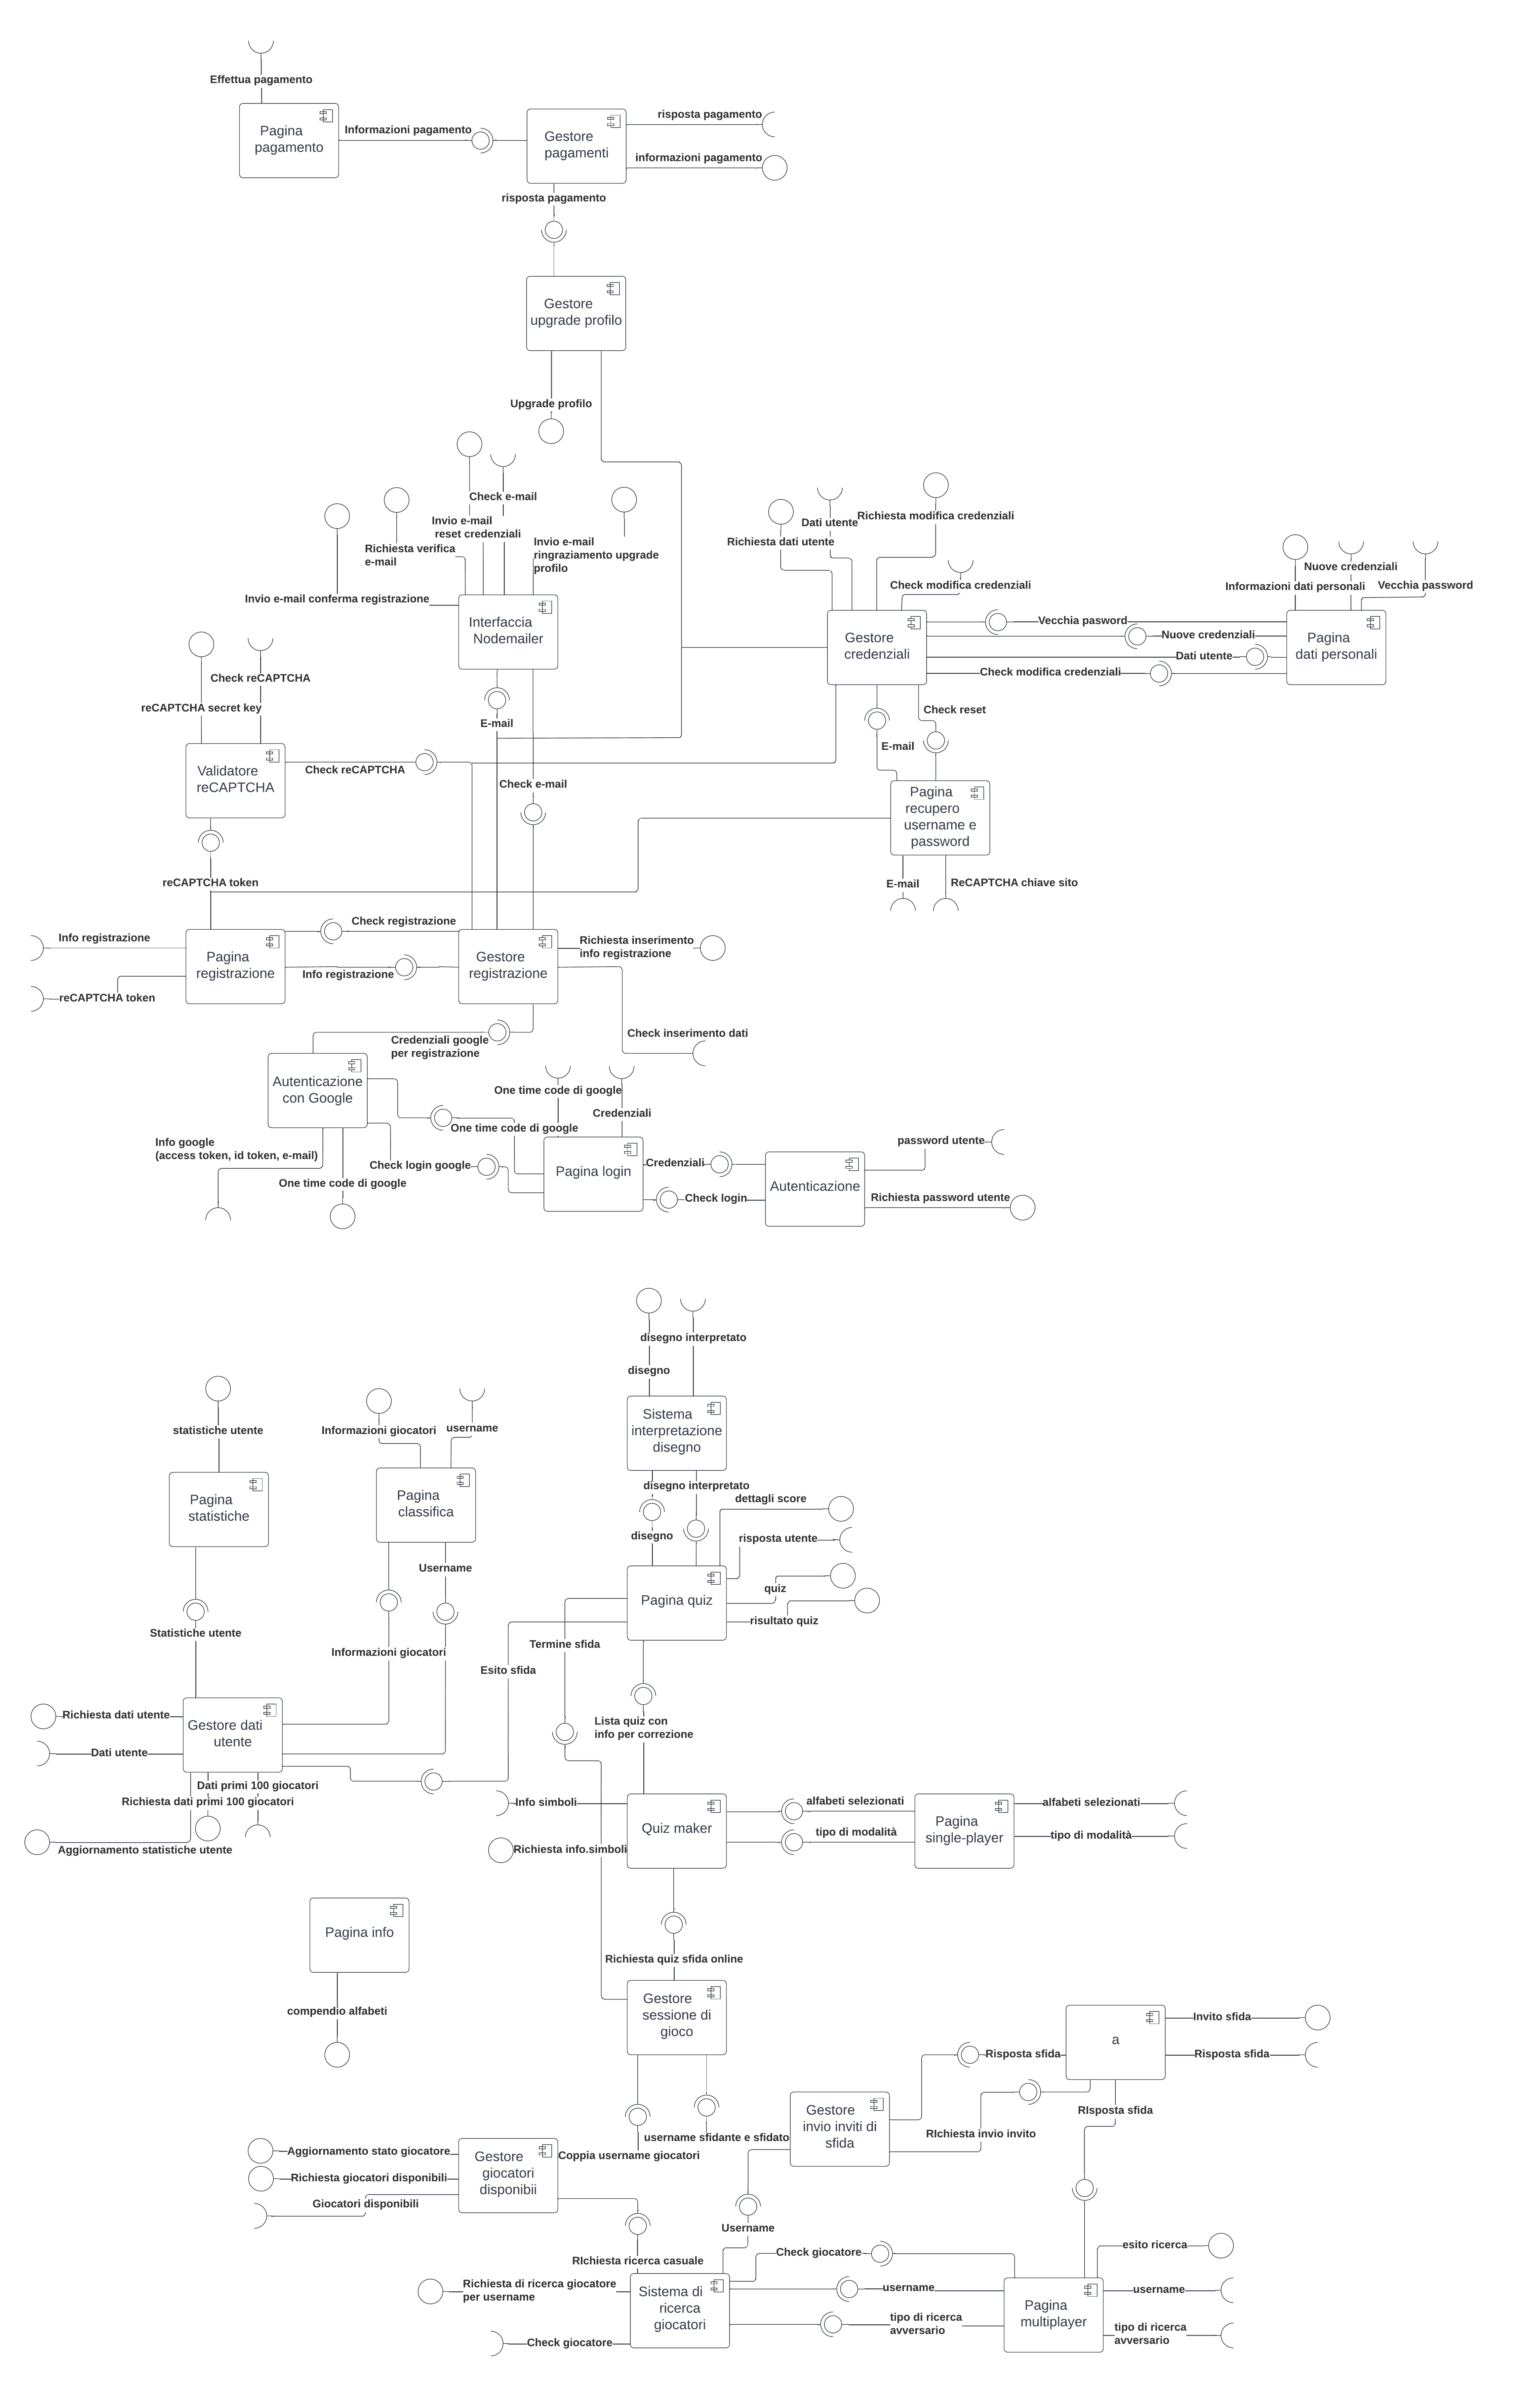
\includegraphics[scale=0.081]{images/diagramma_dei_componenti.png}
\caption{Diagramma dei componenti dell'applicazione JGuesser}
\label{fig:diagramma_dei_componenti}
\end{figure}
\noindent



